\section{Evaluation}
\label{section:evaluation}

\subsection{Methodology}\label{methodology}
We have implemented HashFlow, as well as several latest algorithms that try to improve NetFlow, 
including  FlowRadar\cite{li_flowradar:_2016}, HashPipe\cite{sivaraman_heavy-hitter_2017} 
and ElasticSketch\cite{yang_elastic_2018}, in bmv2 \cite{noauthor_bmv2:_2018}. 
The code for FlowRadar and ElasticSketch are rewritten based on their published code, 
while HashPipe is implemented based on the algorithm in the published paper. As we have implemented HashFlow in a P4 hardware switch\cite{noauthor_edgecore_nodate}, our implementation is strongly constrained due to the resource limitation, so we still use the software switch to evaluate the performance of the algorithms.
%\footnote{The source code has been uploaded to https://github.com/HashFlow with an anonymous account}.

We use 4 traces from different environment to evaluate these algorithms' performance, 
one from a 40 Gbps backbone link provided by CAIDA \cite{noauthor_caida_nodate},
one from a 10 Gbps link in a campus network, and the other two from different ISP access networks.
Some flow level statistics are summarized in Table~\ref{tab:netflowtraces}, 
where we can see that the traffic in different traces differs greatly.
However, by plotting the cumulative flow size distribution in Fig. \ref{fig:flowsizedistribution}, 
we find they all exhibit a similar skewness pattern, 
that most flows are mice flows with a small number of packets, 
while most of the traffic are from a small number of elephant flows \cite{benson_network_2010}.
The only exception is the ISP2 trace, which is 1:5000 sampled from an access link and 
more than 99\% of the flows in it have less than 5 packets (the CDF also reveals this).
When evaluating the algorithms, for each trial, we select a constant number of flows from each trace, 
and feed the packets of these flows to each algorithm. Particularly, since the traces provided by CAIDA and ISP1 are in the granularity of packets while that provided by Campus and ISP2 are in the granularity of flows, the arrival order of packets is determined by the original trace for CAIDA and ISP1 traces, while we generate the packets sequence from the flows randomly for Campus and ISP2 traces.

\begin{table}[ht!]%exp84492
    \centering
    \caption{Traces used for evaluation}
    \label{tab:netflowtraces}
    \begin{tabular} {c | c | c | c }
    \hline\hline
    Trace & Date & max flow size & ave. flow size \\
    \hline
    CAIDA &2018/03/15&92385 pkts & 13.6 pkts\\
    Campus &2014/02/07&289877 pkts & 15.1 pkts\\
    ISP1 &2009/04/10&33003 pkts& 7.5 pkts\\
    ISP2 &2015/12/31&2441 pkts& 1.3 pkts\\
    \hline
    \end{tabular}
\end{table}

\begin{figure}
\centering
\begin{minipage}{.45\linewidth}
    \centering
    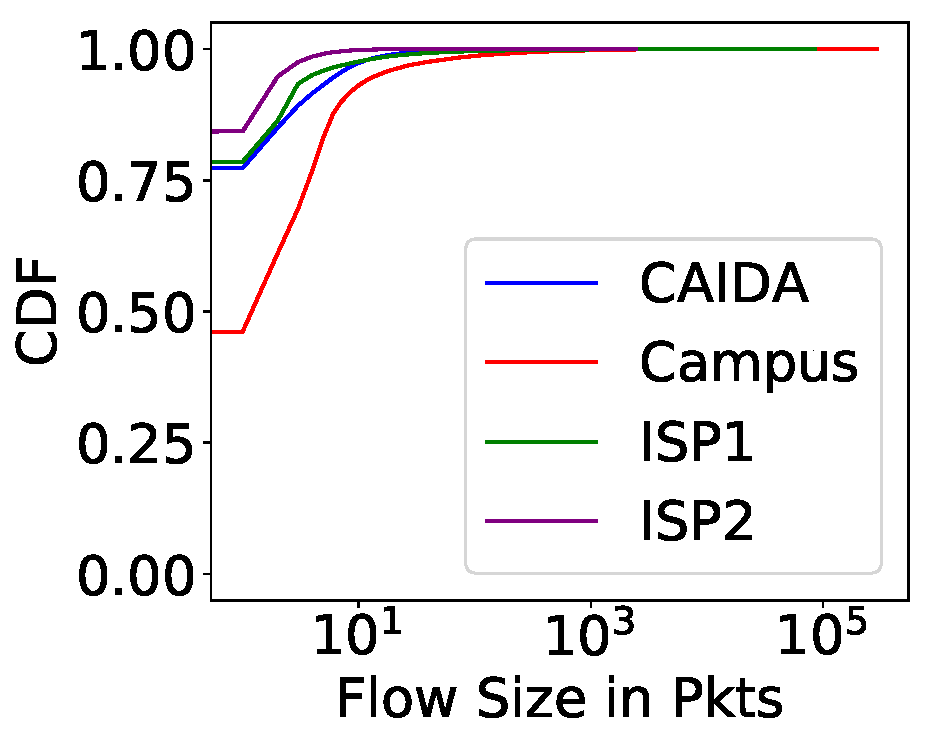
\includegraphics[width=\linewidth]{figures/exp84478/flow_size_distribution}
    \caption{Flow size distribution of the traces used for evaluation}
    \label{fig:flowsizedistribution}
\end{minipage}
\begin{minipage}{.45\linewidth}
	\centering
	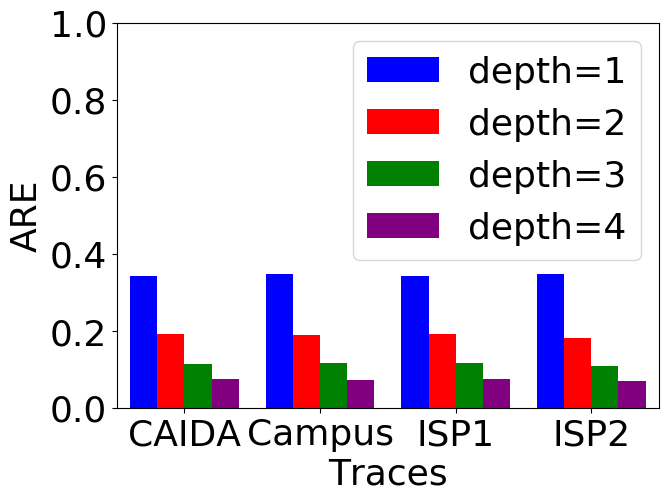
\includegraphics[width=\linewidth]{figures/exp84479/are_with_depth}
	\caption{Flow size estimation under different pipeline depth}
	\label{fig:comparison_increase_depth}
\end{minipage}
\end{figure}

Suppose $n$ flows are processed by each algorithm, where a flow is defined by the typical 5 tuples, i.e., source/destination IP addresses, protocol, and source/destination ports.
The measurement applications we use to evaluate the algorithms 
and traffic statistics we use as performance metrics are as follows. 

\begin{itemize}
    \item \emph{Flow Record Report.} 
An algorithm reports the flow records it maintains, 
where each record is of the form (flow ID, packet count). 
The performance metric we  use is \emph{Flow Set Coverage (FSC)} defined as 
\[FSC\!=\!\frac{\text{num. of flow records with complete flow IDs}}{n}.\]

    \item \emph{Flow Size Estimation.} 
Given a flow ID, an algorithm estimates the number of 
packets belonging to this flow. If no result can be reported, we use 0 as the default value. 
The performance metric we  use is \emph{Average Relative Error (ARE)} defined as 
\[ARE=\frac{1}{n}\sum\left|\frac{\text{estimated size of flow } i }{\text{real size of flow } i}-1\right|.\]

    \item \emph{Heavy Hitter Detection.} 
An algorithm reports heavy hitters, which are flows with more than $T$ packets, 
and $T$ is an adjustable parameter. 
Let $c_1$ be the number of  heavy hitters reported by an algorithm, 
$c_2$ the number of real heavy hitters, 
and among the reported $c_1$ heavy hitters $c$ of them are real.
The performance metric we use is \emph{F1 Score} defined as
\[\text{F1 Score}=\frac{2\cdot PR\cdot RR}{PR + RR},\]
where $PR = \frac{c}{c_1}$  and $RR=\frac{c}{c_2}$. 
We also use \emph{ARE} of the size estimation of the heavy hitters 
as another metric.

    \item \emph{Cardinality Estimation.} 
An algorithm estimates the number of flows. 
The performance metric we  use is \emph{Relative Error (RE)} defined as 
\[RE =\left|\frac{\text{estimated number of flows}}{n}-1\right|.\]
Notice that, linear counting\cite{whang_linear-time_1990} is used by ElasticSketch and HashFlow to estimate the number of flows in the count-min sketch and ancillary table respectively.


\end{itemize}

Following recommendations in the corresponding papers, we set the parameters of these algorithms as follows. 
\begin{itemize}
    \item HashPipe: We use 4 sub-tables of equal size.
    \item ElasticSketch: We adopt the hardware version, where 3 sub-tables
are used in its heavy part. The light part uses a count-min sketch of one array, 
and the two parts use the same number of cells.
    \item FlowRadar:  We use 4 hash functions for its bloom filter and 3 hash functions for its counting table.
The number of cells in the bloom filter is $40\times$ of that in the counting table. 
    \item HashFlow: We use the same number of cells in the main table and the ancillary table. 
The main table consists of three small hash tables with the weight $\alpha$ of 0.7. 
Each digest and counter in the ancillary table costs 8 bits.
\end{itemize}

We let these algorithms use the same amount of memory in all the experiments. 
For each flow record, we use a flow ID of 104 bits and a counter of 32 bits,
So 1 MB memory approximately corresponds to 60K flow records.
In the worst case, HashFlow, HashPipe and ElasticSketch (hardware version) will compute 4 hash results 
to access the corresponding cells, while FlowRadar always needs to compute 7 hash results. To save space, we use the acronyms presented in Table~\ref{table:acronyms} to denote the algorithms in figures when necessary. 

\begin{table}[ht!]
	\centering
	\caption{Acronyms for Algorithms}
	\label{table:acronyms}
	\begin{tabular} { c | c | c | c}
	\hline\hline
	Acronym & Algorithm & Acronym & Algorithm\\
	\hline
	HF & HashFlow & HP & HashPipe\\
%	\hline
%	HP & HashPipe\\
%	\hline
	ES & ElasticSketch & FR & FlowRadar\\
%	\hline
%	FR & FlowRadar\\
	\hline%\hline
	\end{tabular}
\end{table}


%Since we are interested in the flow sizes only, in the implementations we record the flow IDs (including source IP address, destination IP address, protocol, source port and destination port) and flow sizes (in packets) and omit other properties of flows. The data structure of HashFlow consists of 8 register arrays. While it is obvious that the width of five-tuple of flows is 104 bits, we allocate 32 bits to \emph{count} field in MT, 8 bits to \emph{digest} field and \emph{count} field in AT.





\subsection{Optimizing the Main Table and Ancillary Table }
We first demonstrate the performance of the main table with the collision resolution strategy, 
under different settings and parameters, i.e, using a multi-hash table, 
or using pipelined tables with different weights.

In Fig. \ref{fig:performance_comparison_hierarchical_hashtable}, there are 3 pipelined tables of which the weight is 0.6, 0.7 and 0.8 respectively and a multi-hash table. 
The traces are from  the campus network, and we increase the number of flows from 10K to 60K.
It can be seen that the pipelined tables with a weight around $\alpha=0.7$ achieves the best result.
Compared with the multi-hash table, it improves the \emph{FSC} by 3.1\%, 
and reduces the \emph{ARE} by 37.3\% respectively. 
This confirms our theoretical analysis on $\alpha$ in Section \ref{analysis}.
In the experiments thereafter, we will use a default weight of 0.7.


In Fig. \ref{fig:comparison_increase_depth}, we set the number of flow to 50K, and the depth of the main table is set to 1, 2, 3 and 4.
It can be seen that increasing $d$ from 1 to 3 reduces the \emph{ARE} by around 3 times (i.e., from 0.34 to 0.12), 
while increasing $d$ from 3 to 4 will have only a minor improvement (i.e., from 0.12 to 0.075). 
In the experiments thereafter, we will use a default depth of 3.


%As shown in Fig.~\ref{fig:comparison_increase_depth}, as the depth of MT increases from 1 to 4, the ARE (Average Relative Error) of \emph{flow size estimation} decreases from around 0.34 to around 0.075. However, we find that most of the improvement regarding the performance is achieved when the depth increases from 1 to 3 since the ARE is around 0.12 when the depth of MT is 3. Meanwhile, by increasing the depth from 3 to 4, we will have to take the risk of doing one more hash computation and one more memory read operation. so we believe that it is a good tradeoff to constrain the time complexity and give up the benefits of more depths. We will set the default depth of MT to 3. 

\begin{figure}[ht!]
    \centering
    \mbox{
        \subfigure[Flow Record Report\label{MT-flowrecord}]{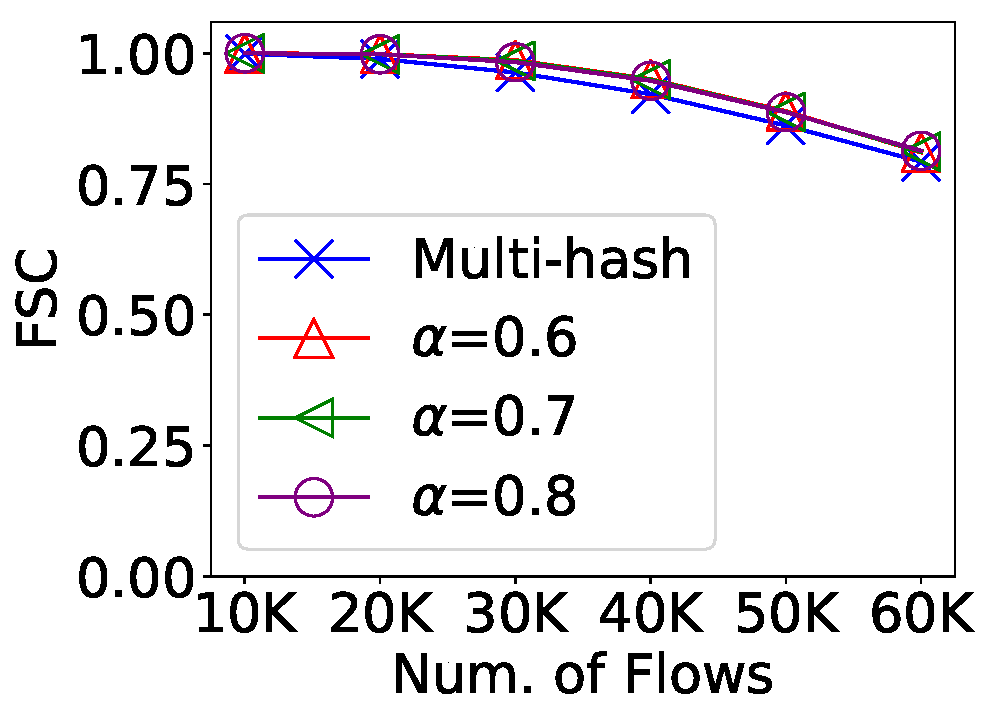
\includegraphics[width=0.45\linewidth]{figures/exp84454/flow_monitoring_fsc}}
        \subfigure[Flow Size Estimation\label{MT-flowsize}]{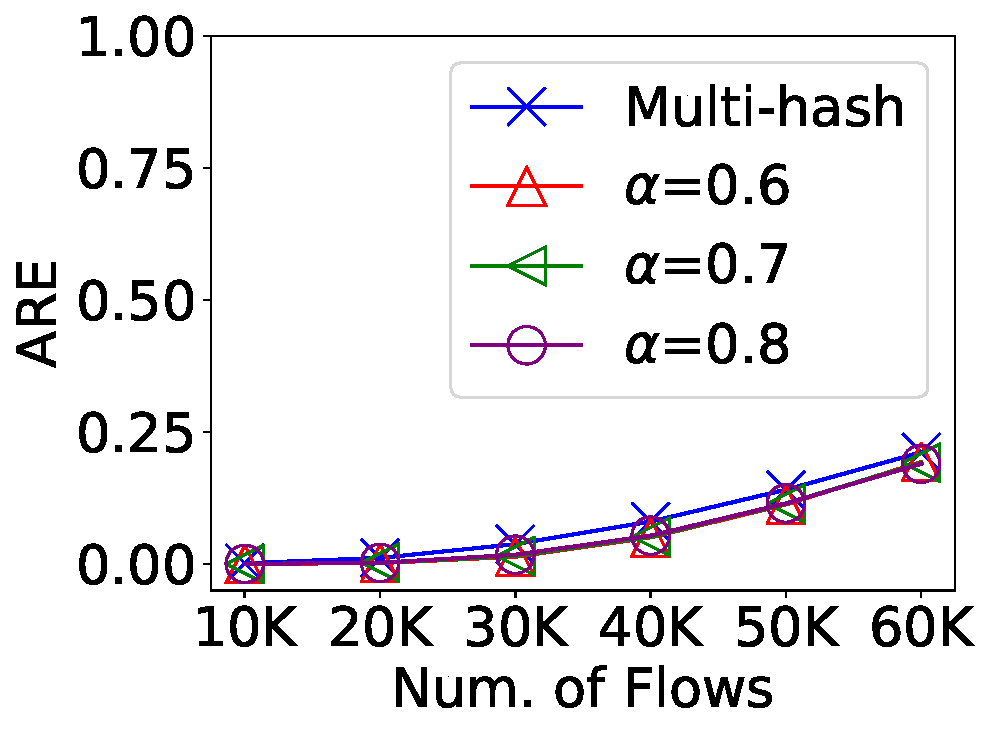
\includegraphics[width=0.45\linewidth]{figures/exp84454/flow_size_estimation_are}}
    }
    \caption{Comparing multi-hash table with pipelined tables.}
    \label{fig:performance_comparison_hierarchical_hashtable}
\end{figure}

To evaluate the influence that the size of ancillary table has upon HashFlow, we define a parameter $\beta$ and let $n_2=n_1\times\beta$, where $n_1$ and $n_2$ are number of buckets in the main table and ancillary table respectively. There is not an ancillary table at all when $\beta=0.0$. We feed a number of flows extracted from CAIDA file, and calculate the F1 Score and ARE (Average Relative Error) of heavy hitter detection where a heavy hitter is a flow with no less than 10 packets. Fig.~\ref{fig:are_for_various_beta} shows that the ancillary table is crucial for the performance of HashFlow and normally $\beta=0.5$ is good enough. However, when attacks such as DDoS occur, the accumulation of elephant flows in ancillary table will be interrupted frequently. To be robust when facing such attacks, in the following experiments we  set $\beta$ to 1.0 by default.

\begin{figure}[ht!]
	\centering
	\mbox{
		\subfigure[F1 Score\label{hhd_f1_score}]{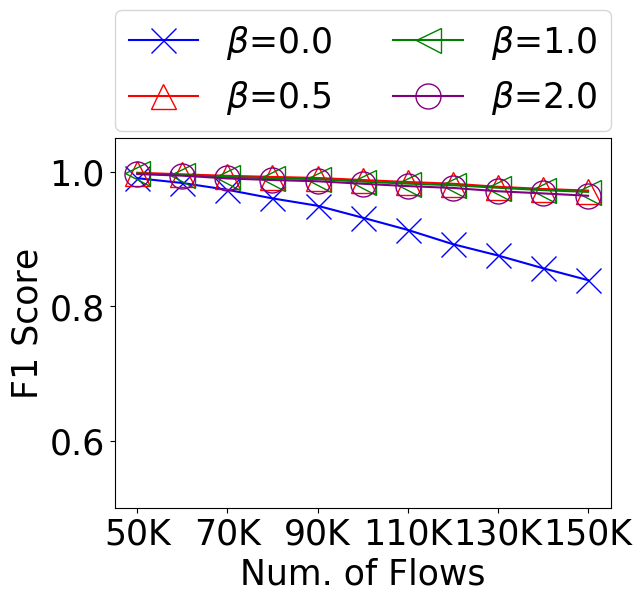
\includegraphics[width=0.45\linewidth]{figures/exp84493/caida_heavy_hitter_detection_f1_score}}
		\subfigure[ARE\label{hhd_ARE}]{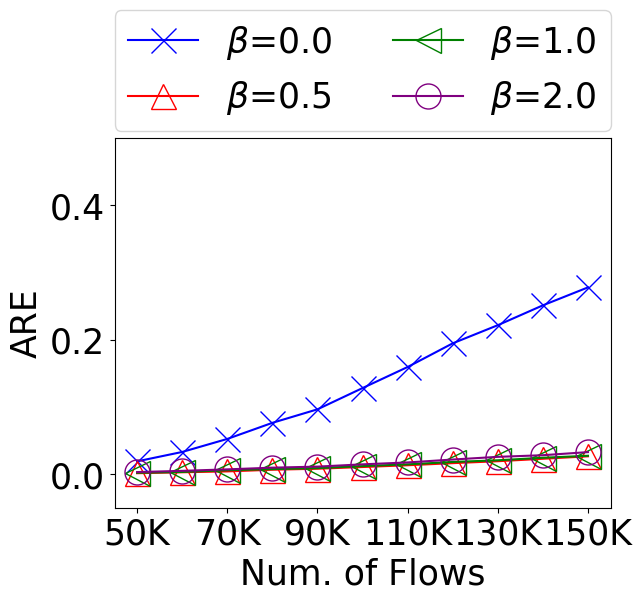
\includegraphics[width=0.45\linewidth]{figures/exp84493/caida_heavy_hitter_detection_are}}
	}
	\caption{F1 Score and Average Relative Error (ARE) of heavy hitter detection when the size of ancillary table varies.}
	\label{fig:are_for_various_beta}
\end{figure}




\subsection{Application Performance }
In this section, we evaluate the performance of HashFlow against HashPipe, ElasticSketch and FlowRadar, 
for typical measurement applications as described in  Section~\ref{methodology}.

Fig.~\ref{fig:comparison_concurrent_flows_increases_flow_monitoring} shows that HashFlow nearly always performs better than the others in the sense of \emph{Flow Set Coverage (FSC)}. For example, 
for a total of 250K flows, it can successfully report around 55K flows, 
nearly making a full use of its main table. 
Its \emph{FSC} is more than 20\% higher than ElasticSketch in all traces, 
and is that higher than HashPipe in the Campus Network trace. 
The only exception when HashFlow loses is that, 
for a very small number of flows (the left up corner in the figures), 
FlowRadar has the highest coverage. 
This is because FlowRadar can successfully decode nearly all flow records when only a few flows arrive. 
But its performance drops significantly soon after the flow count goes beyond a certain point, 
since after that, too many flows mixed up, and the decoding often fails.

\begin{figure*}[ht!]
    \centering
    \mbox{
    \subfigure[CAIDA\label{subfig:caidaflowmonitoring}]{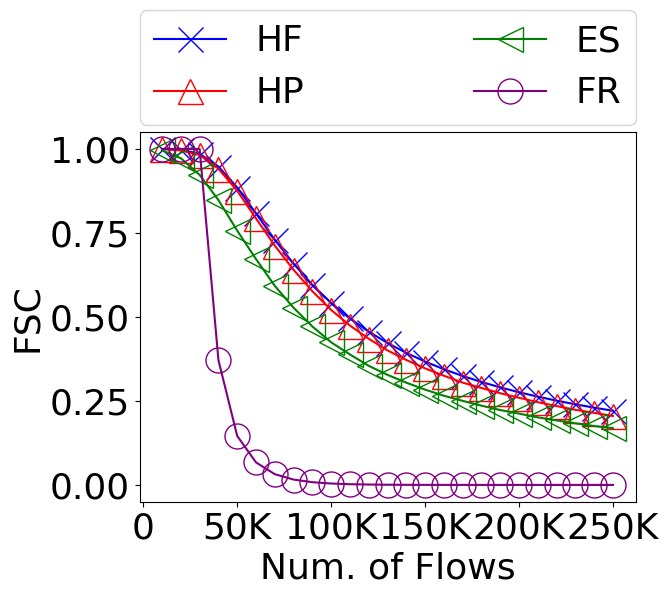
\includegraphics[width=0.24\linewidth]{figures/exp84485/caida_flow_monitoring_fsc}}
    \subfigure[Campus Network\label{subfig:campusnetworkflowmonitoring}]{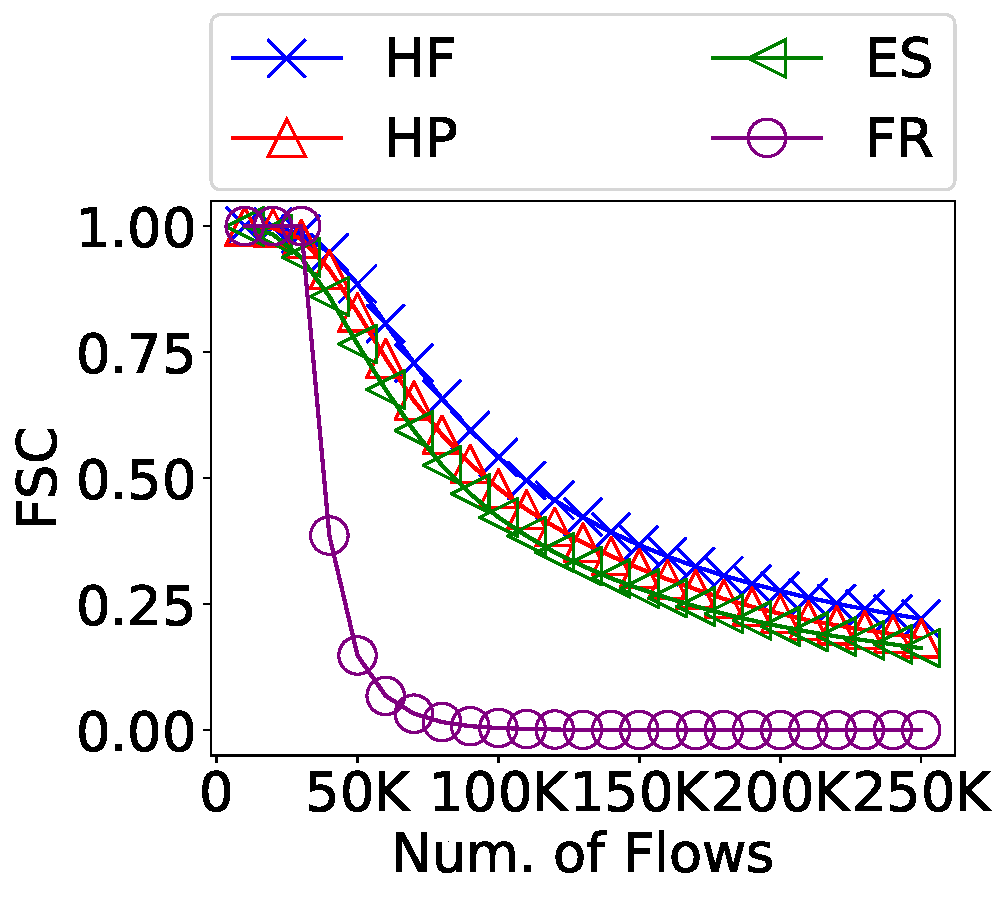
\includegraphics[width=0.24\linewidth]{figures/exp84485/tsinghua_flow_monitoring_fsc}}
    \subfigure[ISP1\label{subfig:hgcflowmonitoring}]{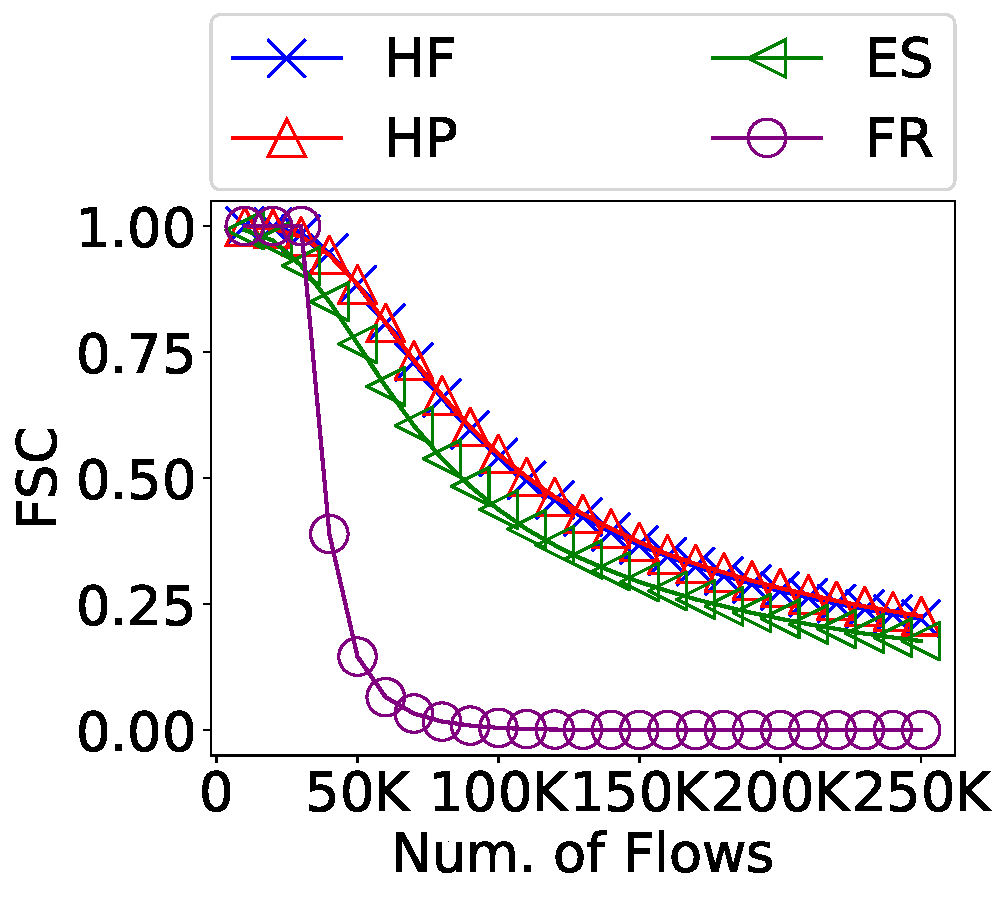
\includegraphics[width=0.24\linewidth]{figures/exp84485/hgc_flow_monitoring_fsc}}
    \subfigure[ISP2\label{subfig:telecomflowmonitoring}]{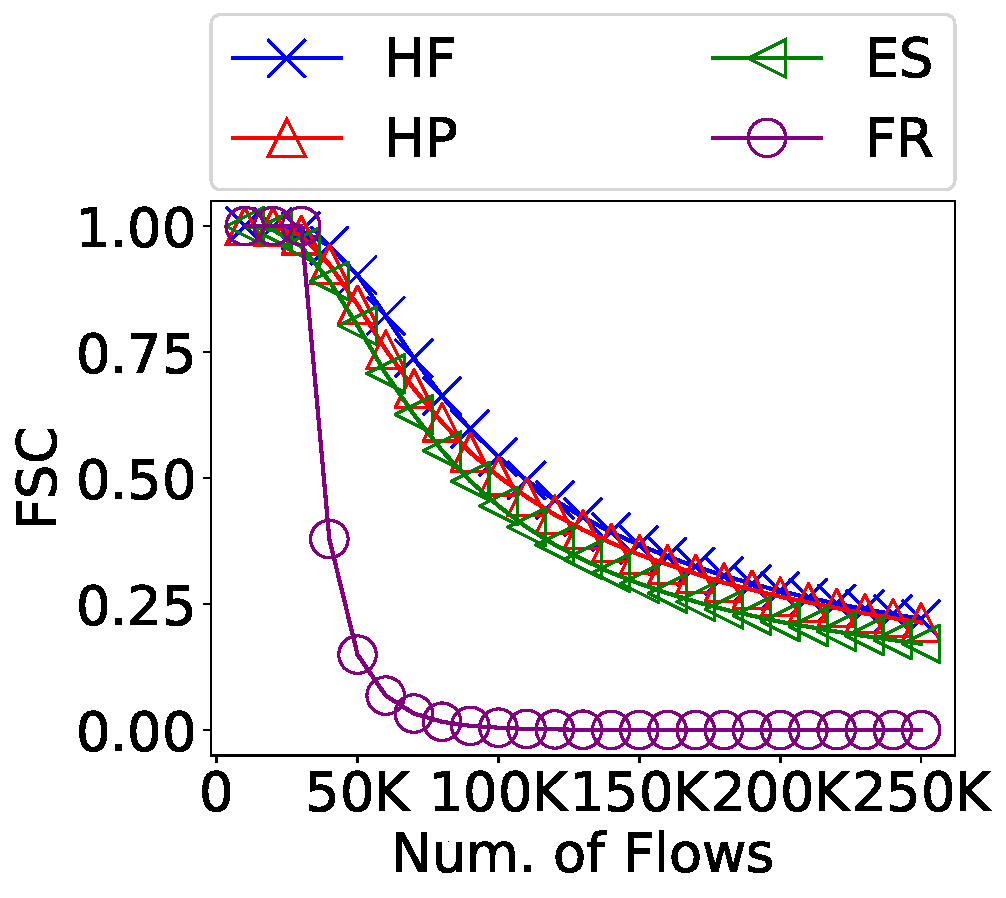
\includegraphics[width=0.24\linewidth]{figures/exp84485/telecom_flow_monitoring_fsc}}
    }
    \caption{\emph{Flow Set Coverage (FSC)} for \emph{Flow Record Report}}
    \label{fig:comparison_concurrent_flows_increases_flow_monitoring}
\end{figure*}

Fig.~\ref{fig:comparison_concurrent_flows_increases_cardinality} shows the results 
of estimating the total number of flows, where in most of the time, 
HashFlow, ElasticSketch and FlowRadar achieve a similar level of accuracy. 
Among them, FlowRadar works slightly better since it uses a bloom filter to count flows, 
which is not sensitive to flow sizes, while HashFlow and ElasticSketch are slightly affected 
by the flow size distribution due to their assumption on the existence of elephant and mice flows. 
This is particularly true in the ISP2 trace, where nearly all flows contain less than 5 packets.
HashPipe always performs badly since it does not use any advanced cardinality estimation technique 
to compensate for the flows it drops. 

\begin{figure*}[ht!]
    \centering
    \mbox{
        \subfigure[CAIDA\label{subfig:caidacardinality}]{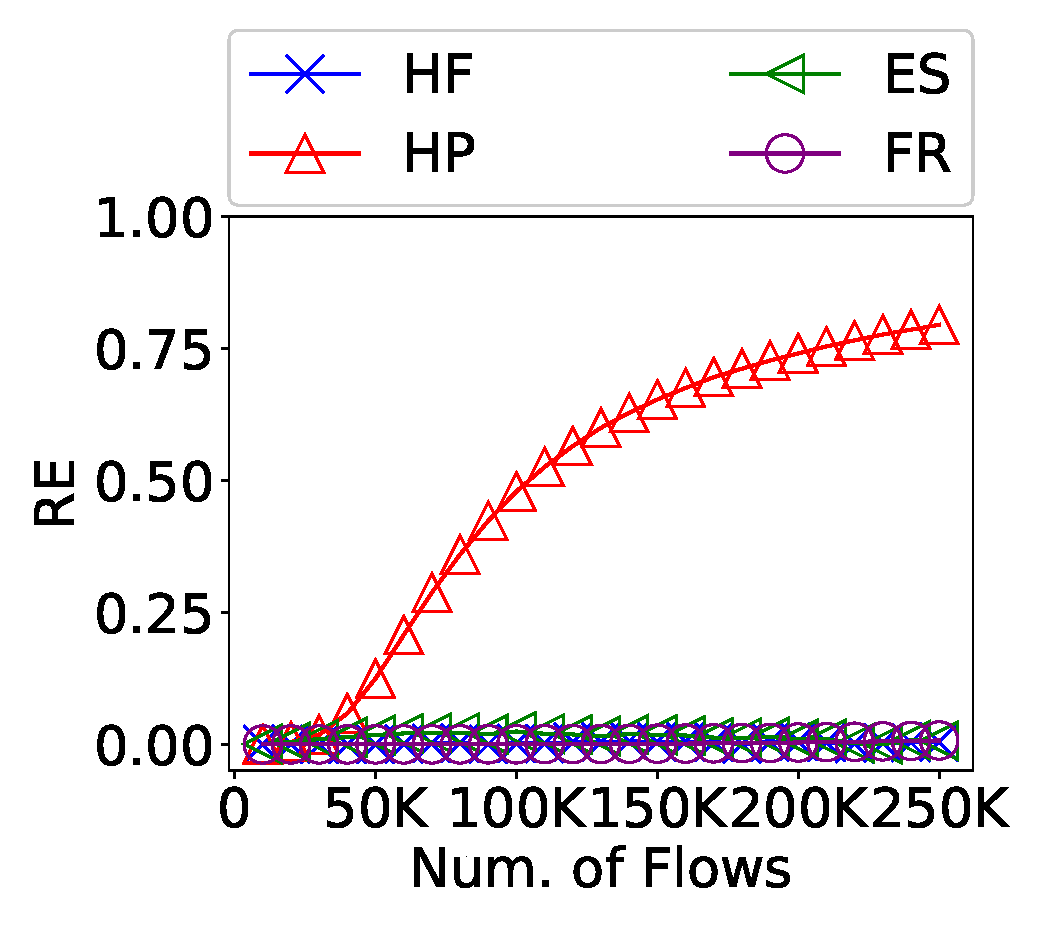
\includegraphics[width=0.24\linewidth]{figures/exp84485/caida_cardinality_re}}
        \subfigure[Campus Network\label{subfig:campusnetworkcardinality}]{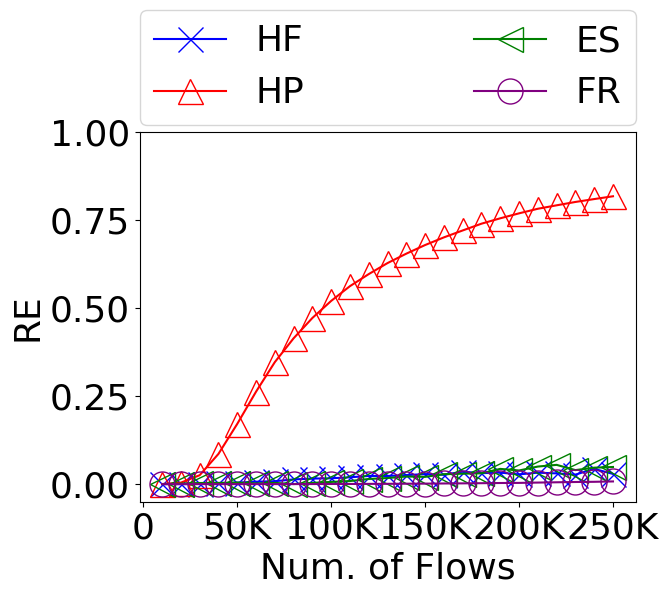
\includegraphics[width=0.24\linewidth]{figures/exp84485/tsinghua_cardinality_re}}
        \subfigure[ISP1\label{subfig:hgccardinality}]{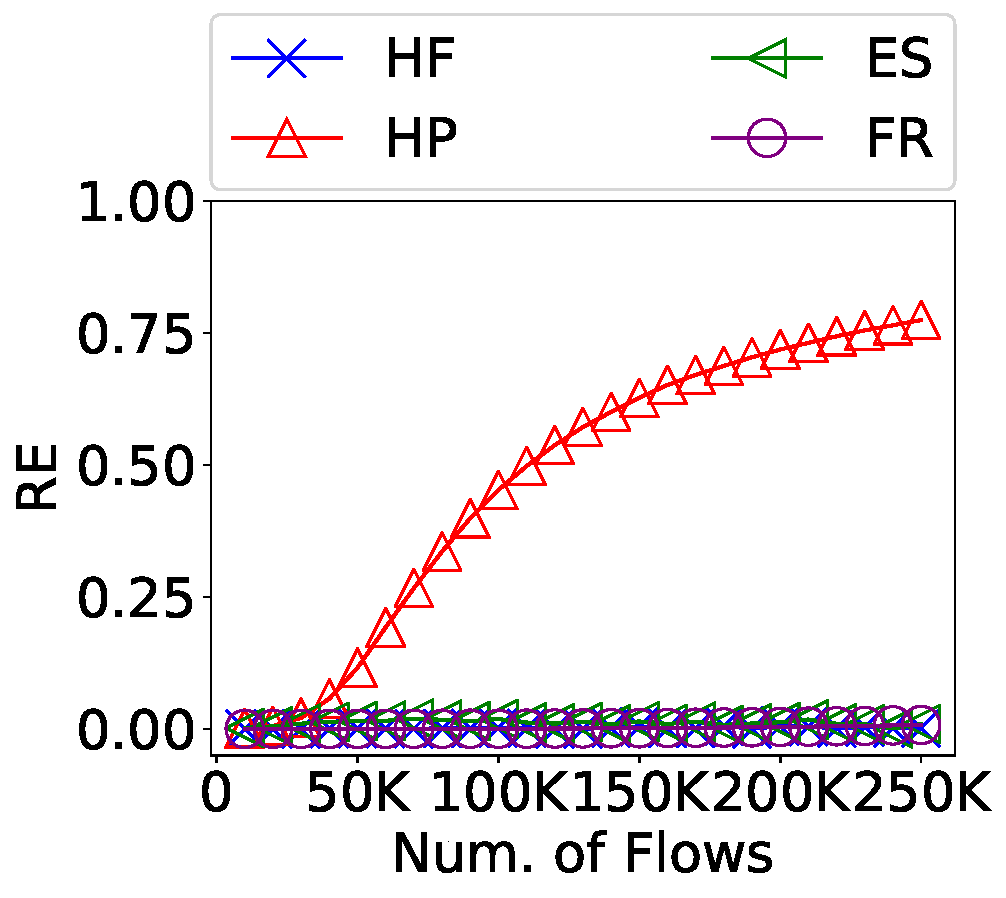
\includegraphics[width=0.24\linewidth]{figures/exp84485/hgc_cardinality_re}}
        \subfigure[ISP2 Trace\label{subfig:telecomcardinality}]{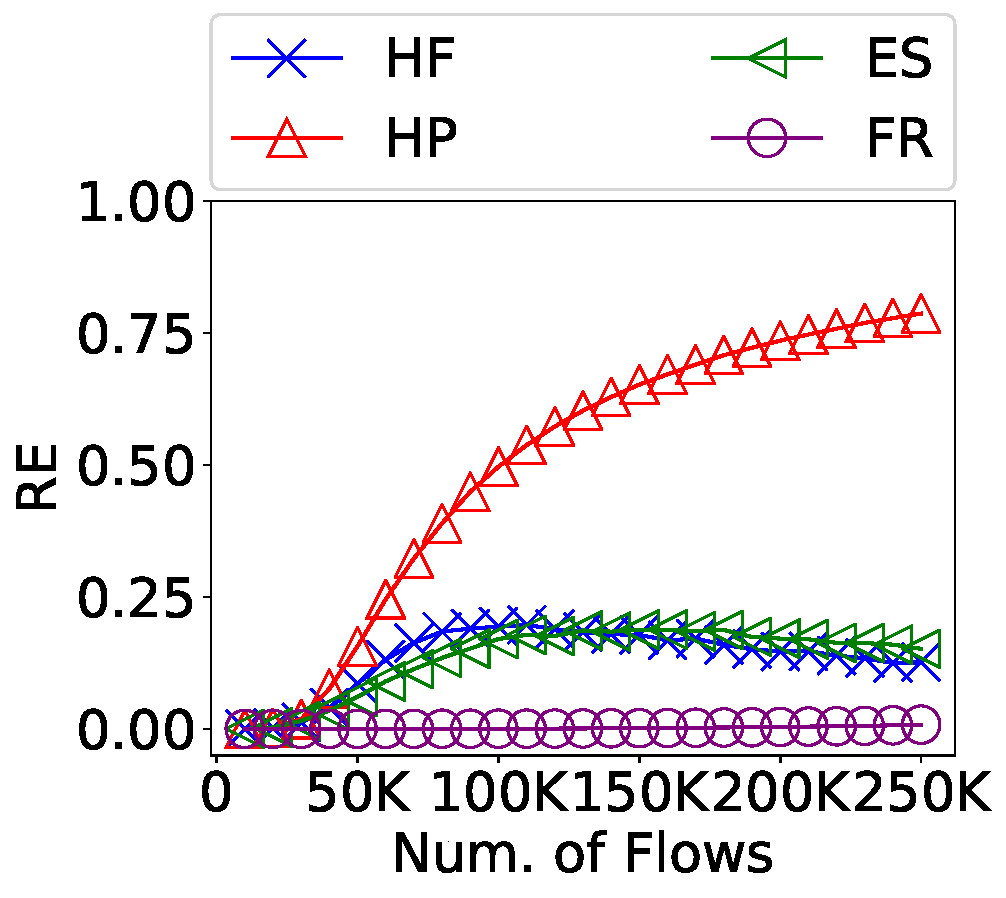
\includegraphics[width=0.24\linewidth]{figures/exp84485/telecom_cardinality_re}}
    }
    \caption{\emph{Relative Error (RE)} for \emph{Flow Cardinality Estimation}}
    \label{fig:comparison_concurrent_flows_increases_cardinality}
\end{figure*}

Fig. \ref{fig:comparison_concurrent_flows_increases_fs_estimation} 
shows that HashFlow often achieves a much lower estimation error 
than its competitors when estimating the flow sizes. For example, when there are 100K flows, the relative estimation error
of HashFlow is around 0.4, while the error of the others is more than 0.6 (50\% higher) in most cases. 
FlowRadar performs very badly when there are more than 40K flows, 
while the accuracy of HashPipe is not very stable.


\begin{figure*}[ht!]
    \centering
    \mbox{
        \subfigure[CAIDA Trace\label{subfig:caidafsestimation}]{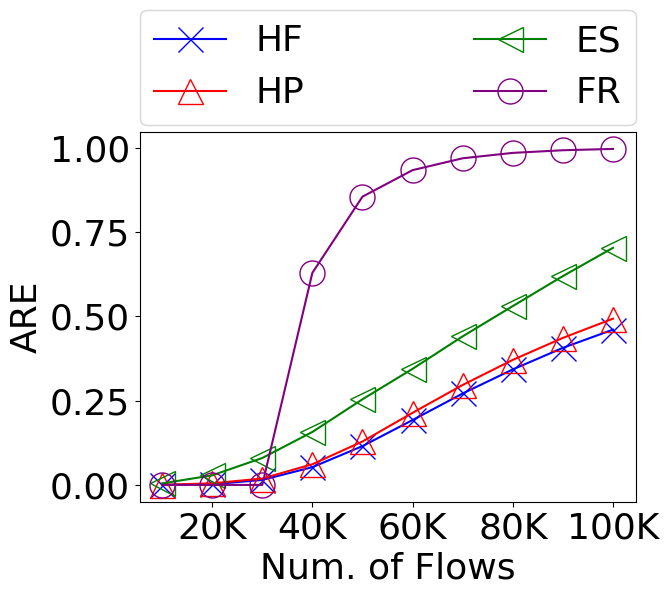
\includegraphics[width=0.24\linewidth]{figures/exp84485/caida_flow_size_estimation_are}}
        \subfigure[Campus Network Trace\label{subfig:campusnetworkfsestimation}]{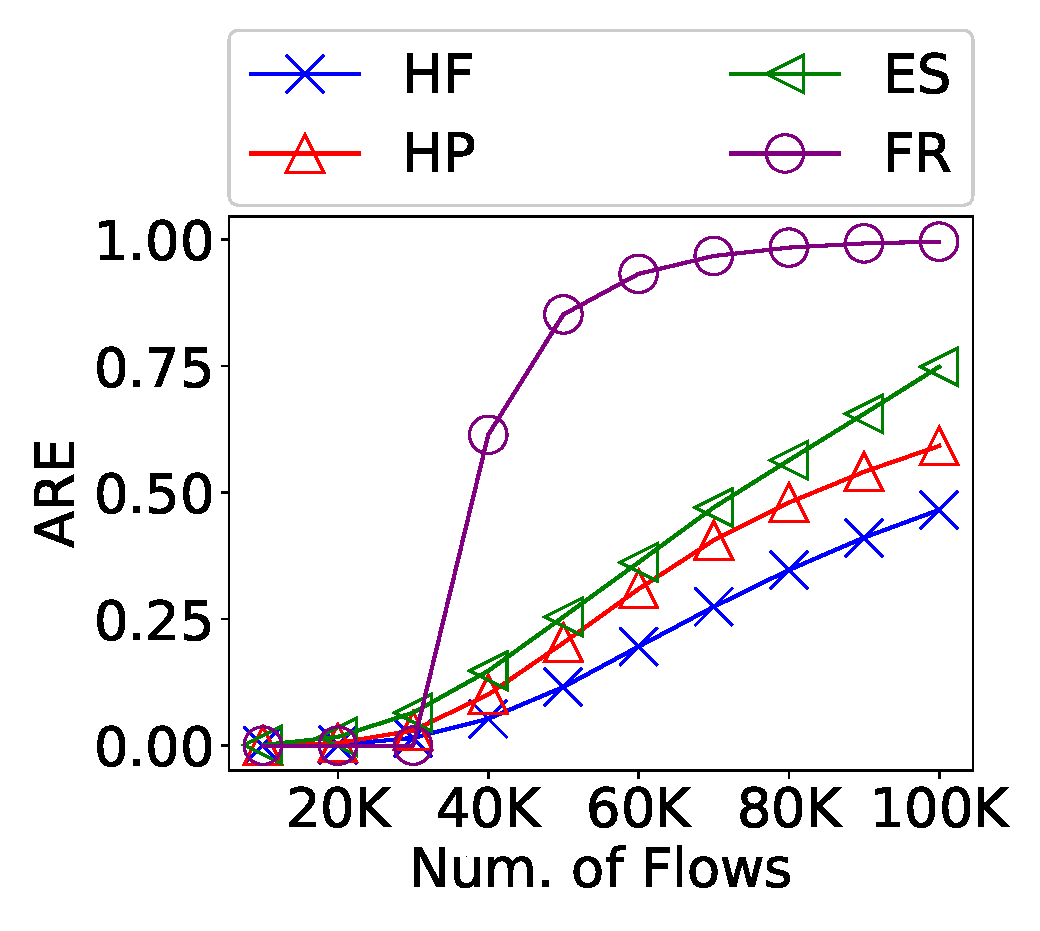
\includegraphics[width=0.24\linewidth]{figures/exp84485/tsinghua_flow_size_estimation_are}}
        \subfigure[HGC Trace\label{subfig:hgcfsestimation}]{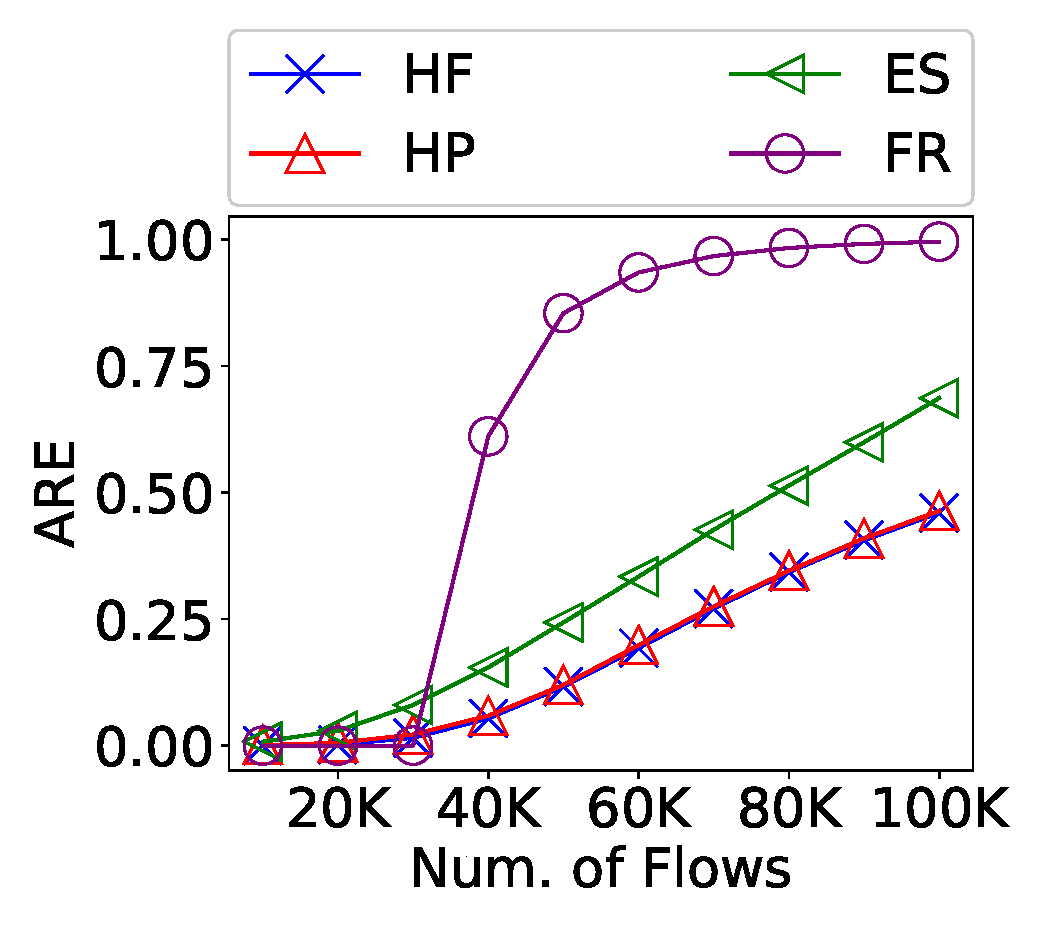
\includegraphics[width=0.24\linewidth]{figures/exp84485/hgc_flow_size_estimation_are}}
        \subfigure[Telecom Trace\label{subfig:telecomfsestimation}]{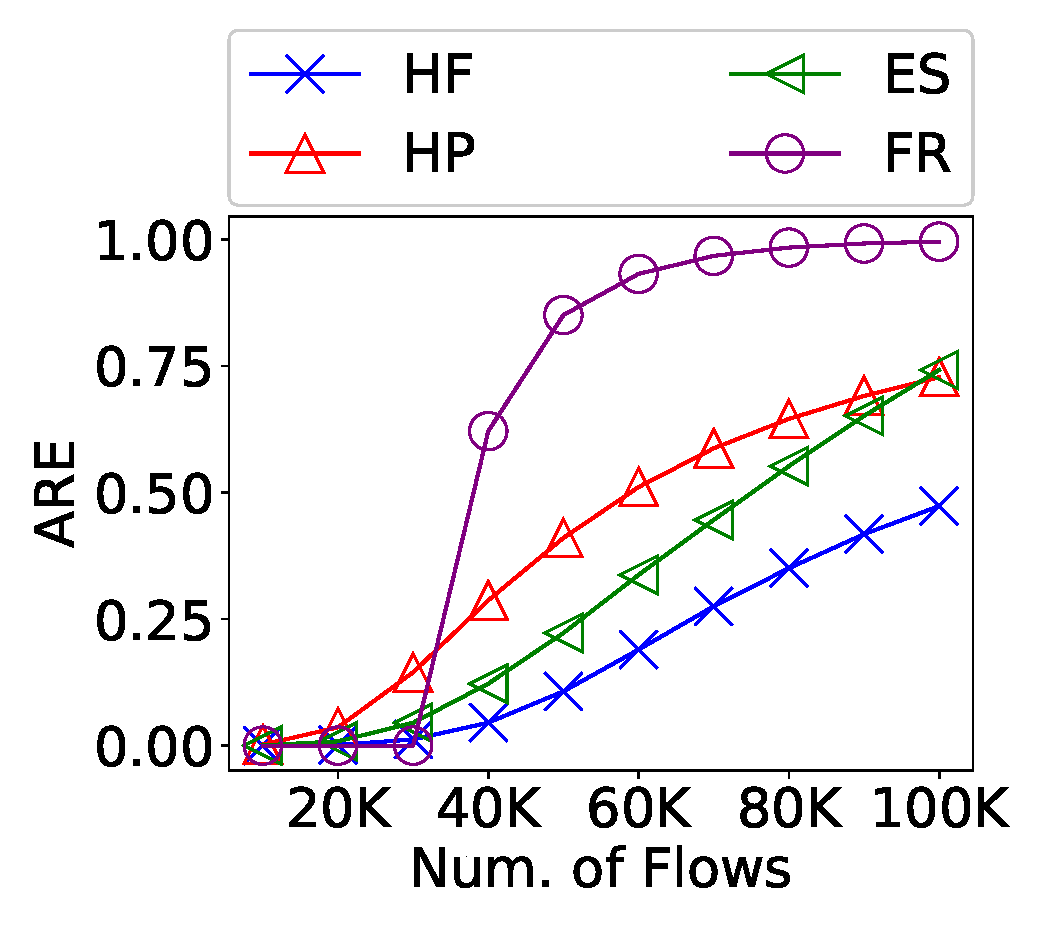
\includegraphics[width=0.24\linewidth]{figures/exp84485/telecom_flow_size_estimation_are}}
    }
    \caption{\emph{Average Relative Error (ARE)} for \emph{Flow Size Estimation}}
    \label{fig:comparison_concurrent_flows_increases_fs_estimation}
\end{figure*}

At last, we show whether they can accurately detect heavy hitters.
We feed 250K flows to each algorithm, and calculate the \emph{F1 Score} of their detection accuracy as well as the $ARE$ of the estimated sizes of the detected heavy hitters.
%where the threshold for a flow to be treated as a heavy hitter varies. 
The results are depicted in Fig. \ref{fig:comparison_concurrent_flows_increases_hhd_f1_score} 
and Fig.~\ref{fig:comparison_concurrent_flows_increases_hhd_are}, respectively. 
Apparently, FlowRadar is not a good candidate under such heavy load. 
HashPipe is designed specifically for detecting heavy hitters, 
but our HashFlow still outperforms it in nearly all cases, for both metrics. 
Not considering the extreme case of the ISP2 trace where most flows are typically very small, 
for a wide range of thresholds, HashFlow achieves a \emph{F1 Score} of 1 (accurately detecting all heavy hitters) 
when the scores of HashPipe and ElasticSketch are around 0.9 and 0.4 $\sim$ 0.7, respectively. 
On the other hand, when HashFlow makes nearly perfect size estimation of the heavy hitters, 
the \emph{ARE} of HashPipe and ElasticSketch are around 0.15 $\sim$ 0.2 and 0.2 $\sim$ 0.25, respectively.
Even with a very small threshold used in the ISP2 trace, HashFlow clearly outperforms the others.

\begin{figure*}[ht!]
    \centering
    \mbox{
        \subfigure[CAIDA\label{subfig:caidahhdf1score}]{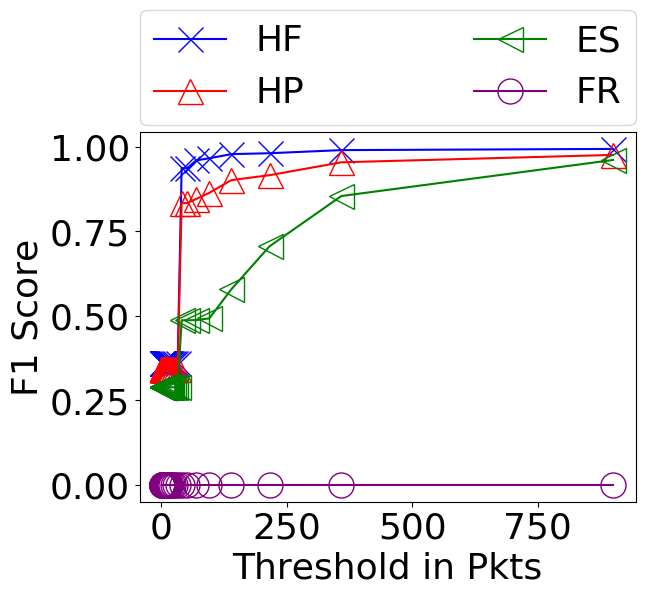
\includegraphics[width=0.24\linewidth]{figures/exp84486/caida_250K_f1_score}}
        \subfigure[Campus Network\label{subfig:campusnetworkhhdf1score}]{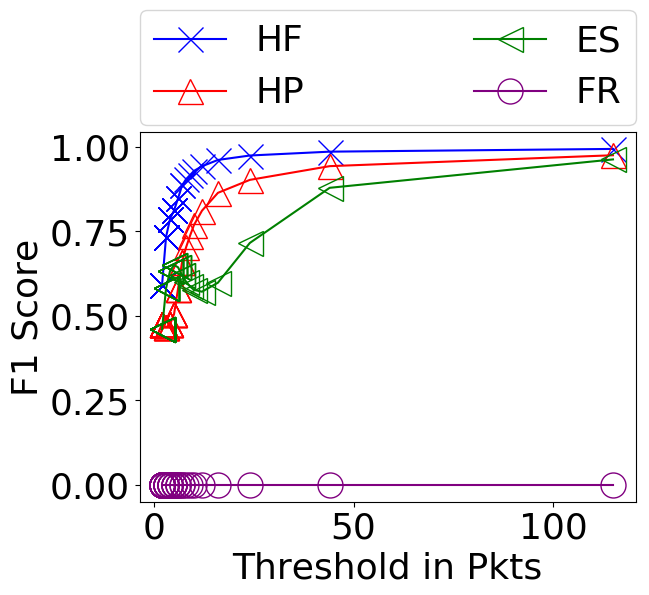
\includegraphics[width=0.24\linewidth]{figures/exp84486/tsinghua_250K_f1_score}}
        \subfigure[ISP1\label{subfig:hgchhdf1score}]{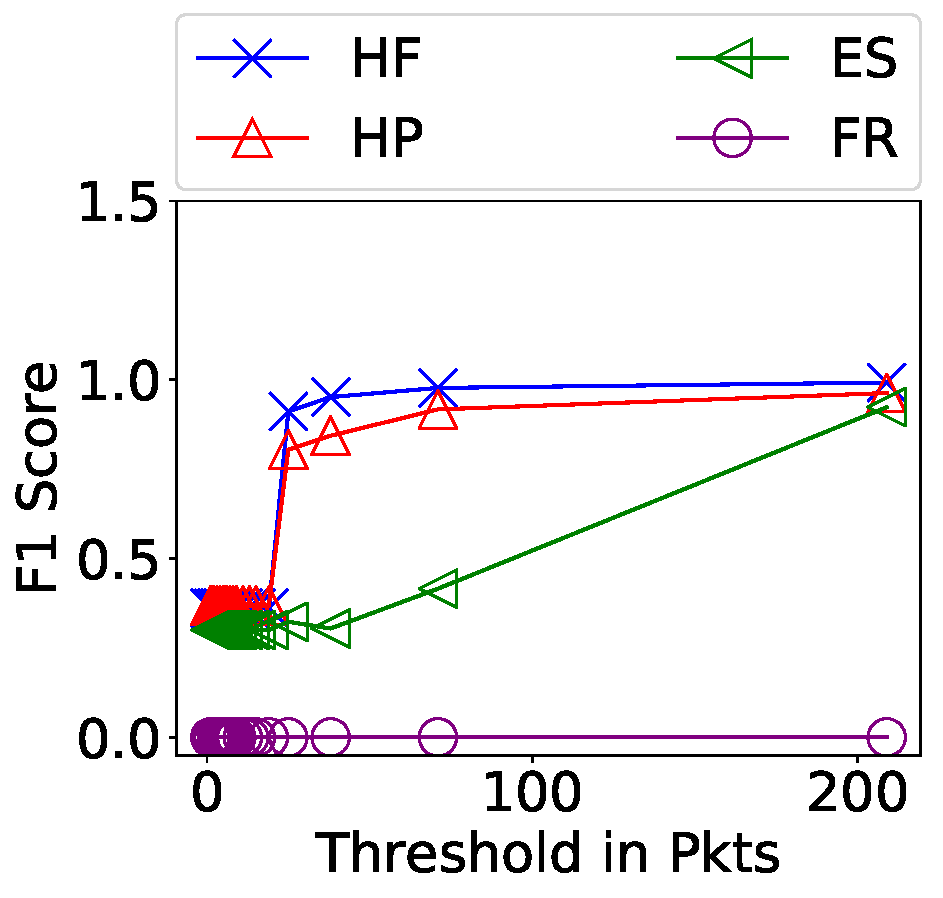
\includegraphics[width=0.24\linewidth]{figures/exp84486/hgc_250K_f1_score}}
        \subfigure[ISP2\label{subfig:telecomhhdf1score}]{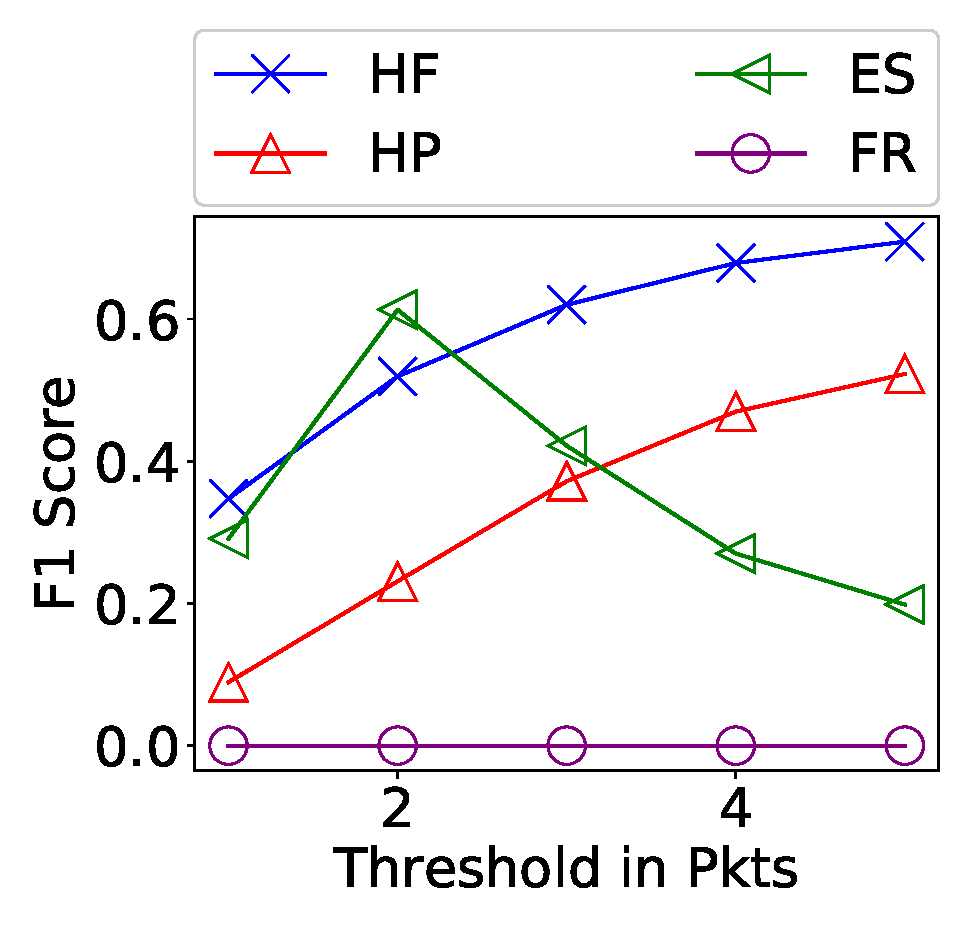
\includegraphics[width=0.24\linewidth]{figures/exp84486/telecom_250K_f1_score}}
    }
    \caption{\emph{F1 Score} for \emph{Heavy Hitter Detection}}
    \label{fig:comparison_concurrent_flows_increases_hhd_f1_score}
\end{figure*}


\begin{figure*}[ht!]
    \centering
    \mbox{
        \subfigure[CAIDA\label{subfig:caidahhdare}]{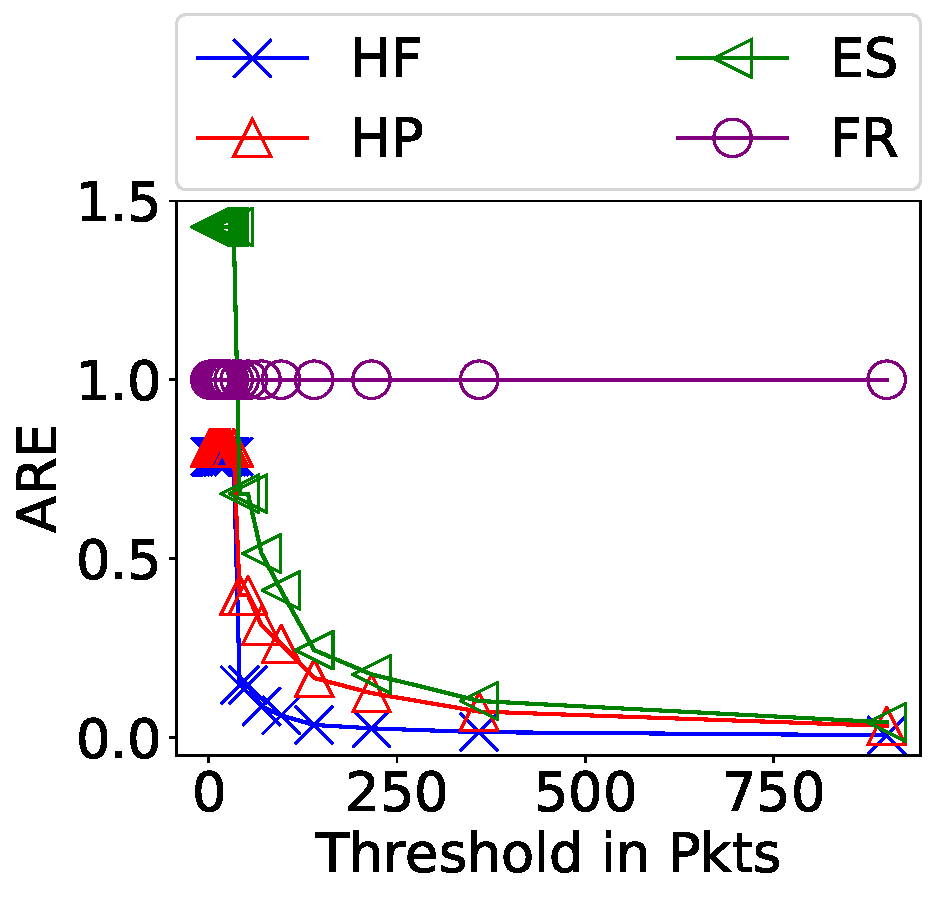
\includegraphics[width=0.24\linewidth]{figures/exp84486/caida_250K_re}}
        \subfigure[Campus Network\label{subfig:campusnetworkhhdare}]{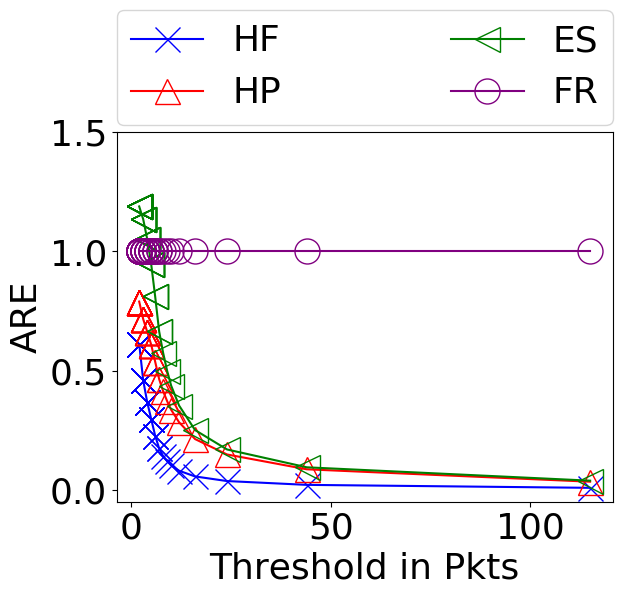
\includegraphics[width=0.24\linewidth]{figures/exp84486/tsinghua_250K_re}}
        \subfigure[ISP1\label{subfig:hgchhdare}]{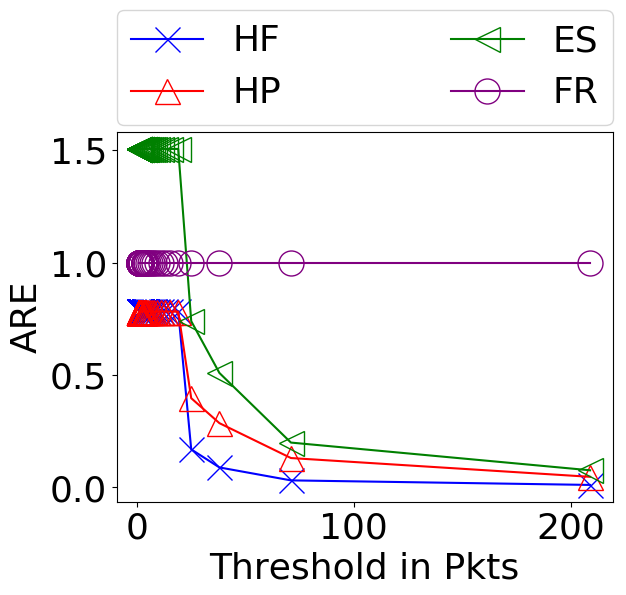
\includegraphics[width=0.24\linewidth]{figures/exp84486/hgc_250K_re}}
        \subfigure[ISP2\label{subfig:telecomhhdare}]{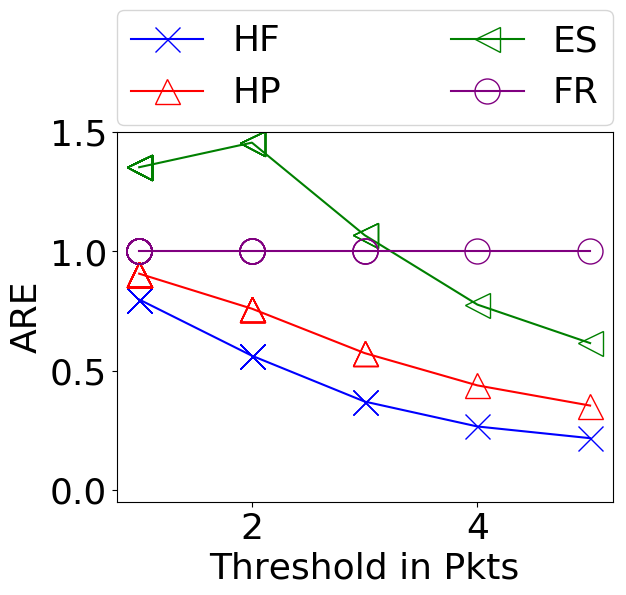
\includegraphics[width=0.24\linewidth]{figures/exp84486/telecom_250K_re}}
    }
    \caption{\emph{Average Relative Error(ARE)} for \emph{Heavy Hitter Detection}}
    \label{fig:comparison_concurrent_flows_increases_hhd_are}
\end{figure*}

\subsection{Throughput}
\label{subsec:throughput}
\begin{figure*}[ht!]
	\centering
	\mbox{
		\subfigure[Throughput\label{fig:throughput}]{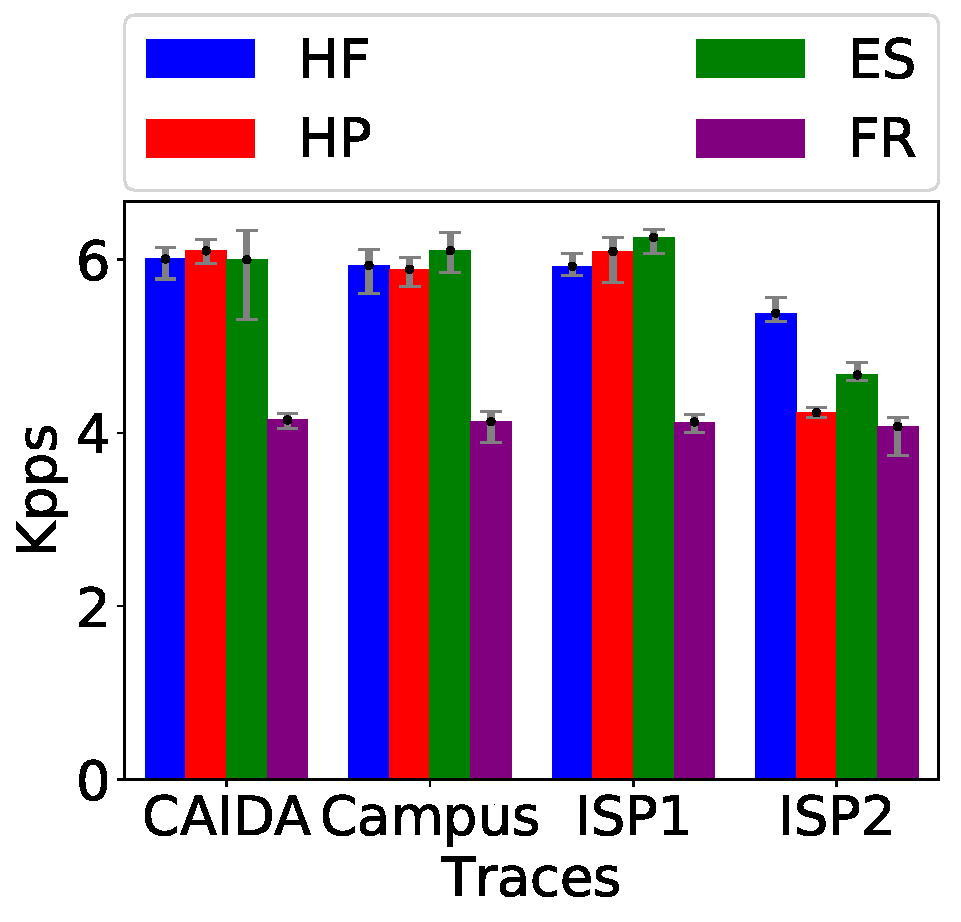
\includegraphics[width=0.24\linewidth]{figures/exp84484/throughput}}
		\subfigure[Number of hash operations\label{fig:avehash}]{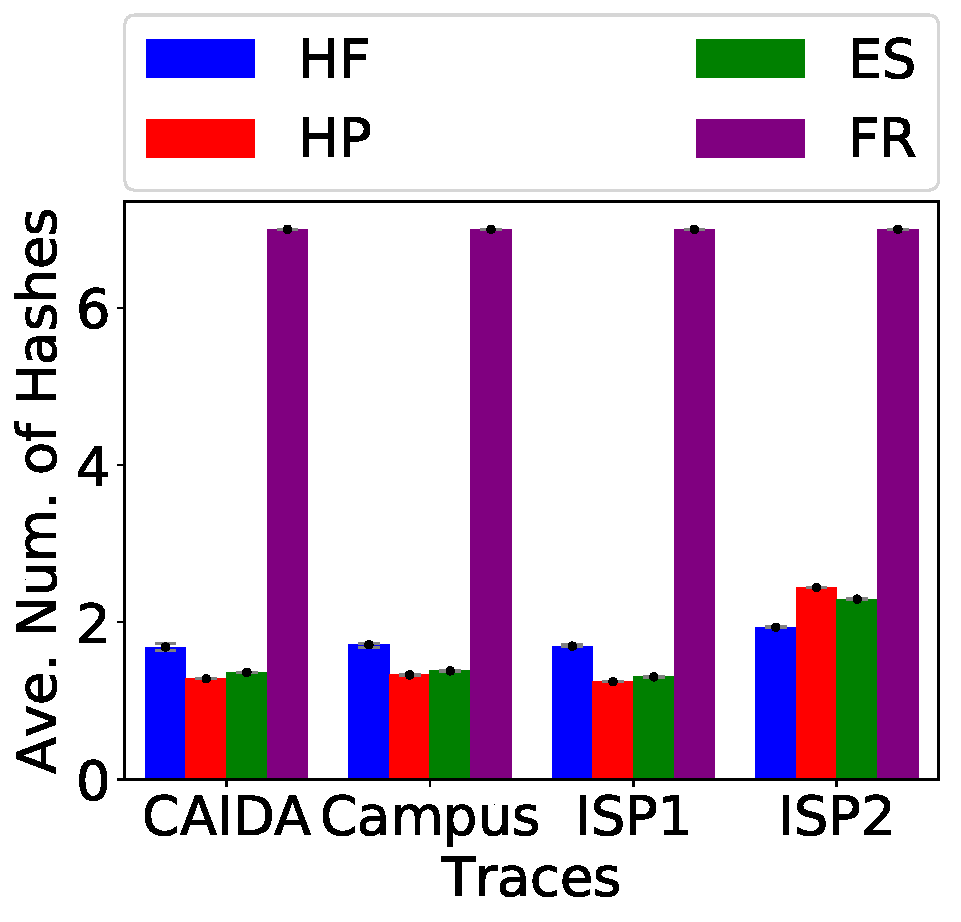
\includegraphics[width=0.24\linewidth]{figures/exp84490/ave_hash}}
		\subfigure[Number of memory accesses\label{fig:avemem}]{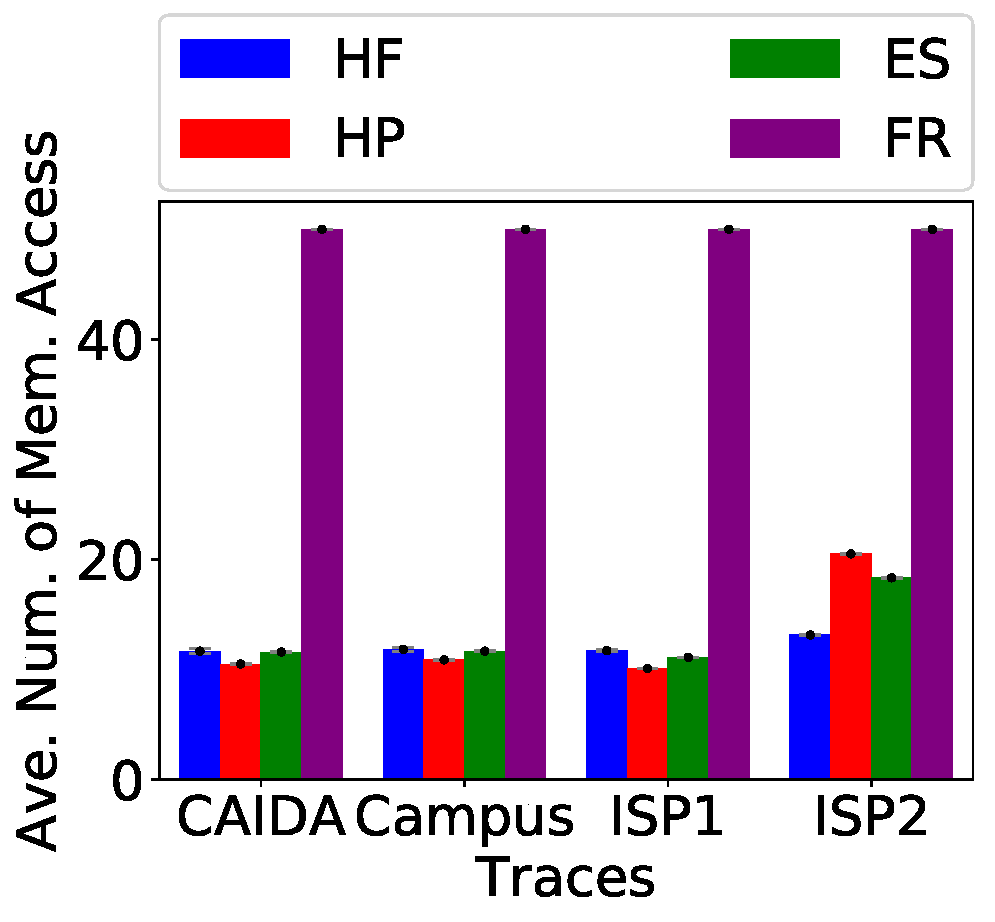
\includegraphics[width=0.24\linewidth]{figures/exp84490/ave_mem}}
		\subfigure[Resubmit Rate\label{fig:increaseinprocessing}]{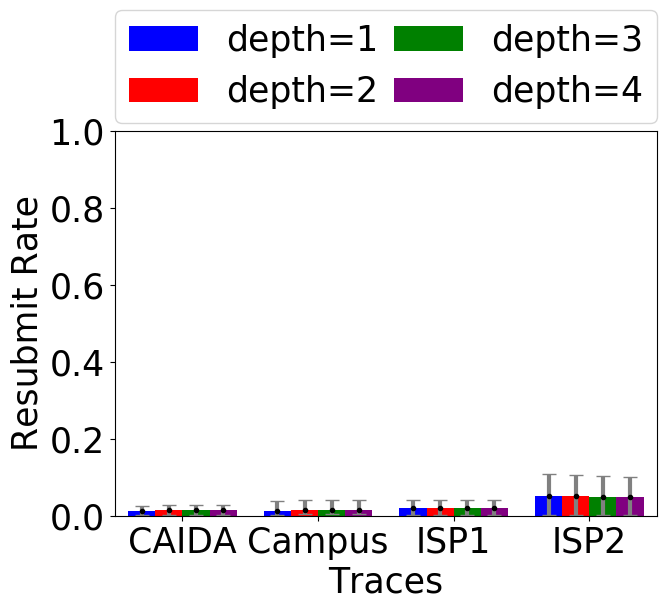
\includegraphics[width=0.24\linewidth]{figures/exp84491/increase_in_processing}}
	}
	\caption{Throughput, Hash Operation, Memory Access and Increase in Processing}
	\label{throughput}
\end{figure*}
We test the throughput of these algorithms with bmv2, 
on a PC with Intel(R) Core(TM) i5-4680K CPU@3.40GHz, 
where each CPU core owns a 6144 KB cache. 
We  use \emph{isolcpus} to isolate the cores to prevent context switches.
Bmv2 achieves around 20 Kpps forwarding speed, 
and the throughput after loading the algorithms are depicted in Fig. \ref{fig:throughput}.
To obtain a better understanding, we also record the average number of 
hash operations, as well as memory accesses, for each algorithm. 
The  results in Fig. \ref{fig:avehash} and Fig. \ref{fig:avemem} indicate that, 
HashFlow will perform comparably to HashPipe and ElasticSketch, 
and much better than FlowRadar, in the sense of the number of memory accesses and hash operations.

In our hardware implementation, the only risk degrading the throughput of the switch is that some packets will be resubmitted (or recirculated), so the switch will have to process more packets than those transmitted through it. To evaluate the possible loss of throughput, we calculate the \emph{Resubmit Rate} defined as 
%$\text{Resubmission Rate}=\frac{n_2}{n_1}.$
\begin{eqnarray*}
\text{Resubmit Rate}=\frac{n_2}{n_1}.
\end{eqnarray*}
where $n_1$ is the number of packets arriving at the switch, and $n_2$ is the number of packets that are resubmitted.

As shown in Fig.~\ref{fig:increaseinprocessing}, when there are 100K flows fed into the switch, the \emph{Resubmit Rate} is normally less than 2\%, and it is no more than 5.2\% in the trace provided by ISP2, which is far less skewed than the real network traffic. So HashFlow will achieve very good performance and the loss of throughput is negligible.


%calculate the average number of memory accesses and hash computations for processing a packet. As shown in Fig.~\ref{fig:avehash}, the average number of hash computations of HashFlow is slightly greater than the other 3 algorithms on the first 3 traces. For example, the average number of computations of HashFlow is 23.5\% and 31.2\% greater than that of ElasticSketch and HashPipe respectively on the CAIDA trace. That's because ElasticSketch and HashPipe allows a flow record to be cached in multiple positions of the data structure, so a elephant flow is more likely to be cached in the starting sub-tables, avoiding making more hash computations and traversing deep into the sub-tables, while a elephant stored the the last sub-table by HashFlow will always be there. This can be proved by the fact that HashFlow needs fewer hash computations on the trace of ISP2, where the elephant flows contribute relatively small part of the packets. Another finding is that the difference in the number of memory accesses is smaller than the difference in the number of hash computations between HashFlow and other algorithms on the first 3 traces. For example, the average number of memory accesses of HashFlow is 10.5\% and 0.6\% greater than that of HashPipe and ElasticSketch, which is far less than the difference in the number of hash computations. That's because ElasticSketch and HashPipe need to repeatedly write into the memory when processing a packet, while HashFlow need to write into the memory only once. 


\iffalse
%\begin{figure}[ht!]
%    \centering
%    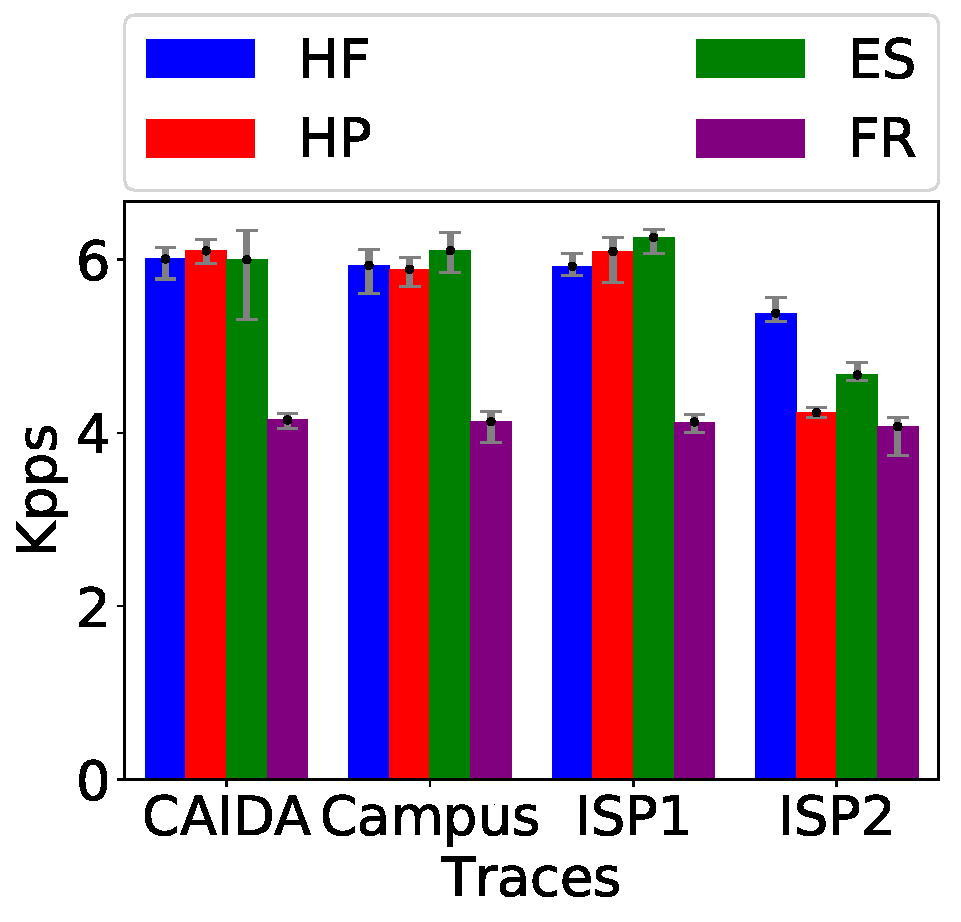
\includegraphics[width=0.9\linewidth]{figures/exp84484/throughput}
%    \caption{The throughput of the algorithms on the four traces.}
%    \label{fig:throughput}
%\end{figure}

%\begin{figure}
%    \centering
%    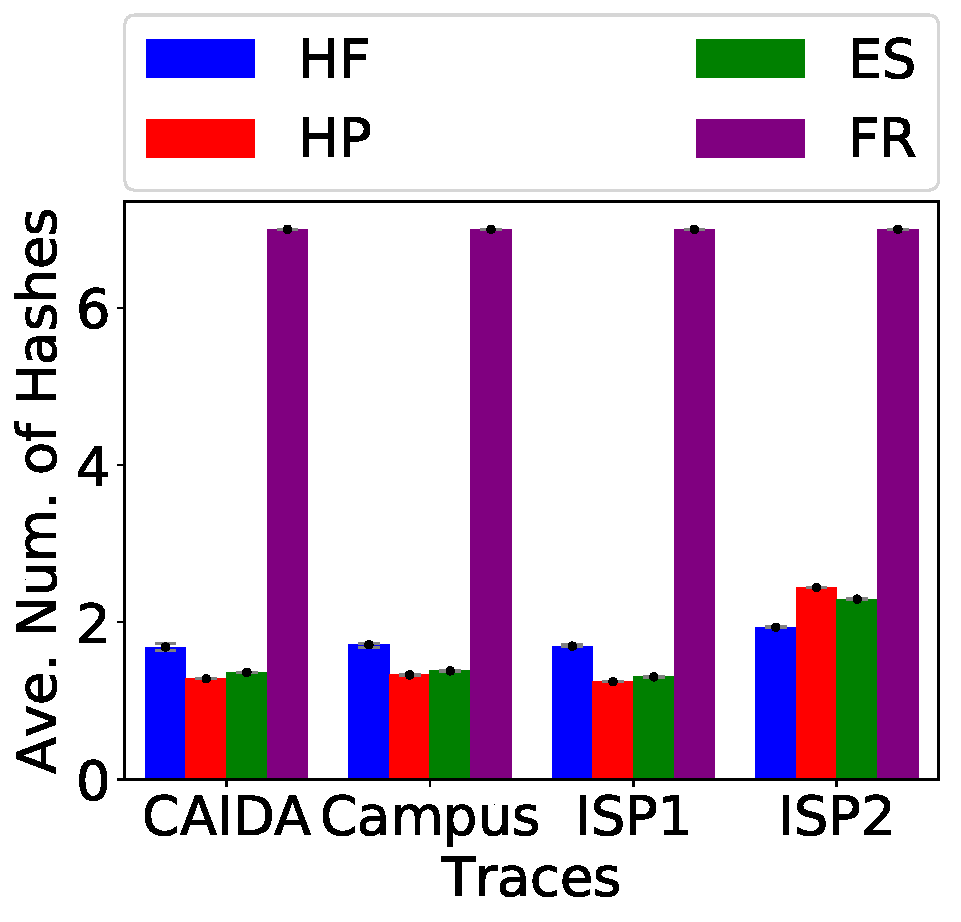
\includegraphics[width=0.9\linewidth]{figures/exp84490/ave_hash}
%    \caption{The average number of hashes for processing a packet.}
%    \label{fig:avehash}
%\end{figure}

%\begin{figure}
%    \centering
%    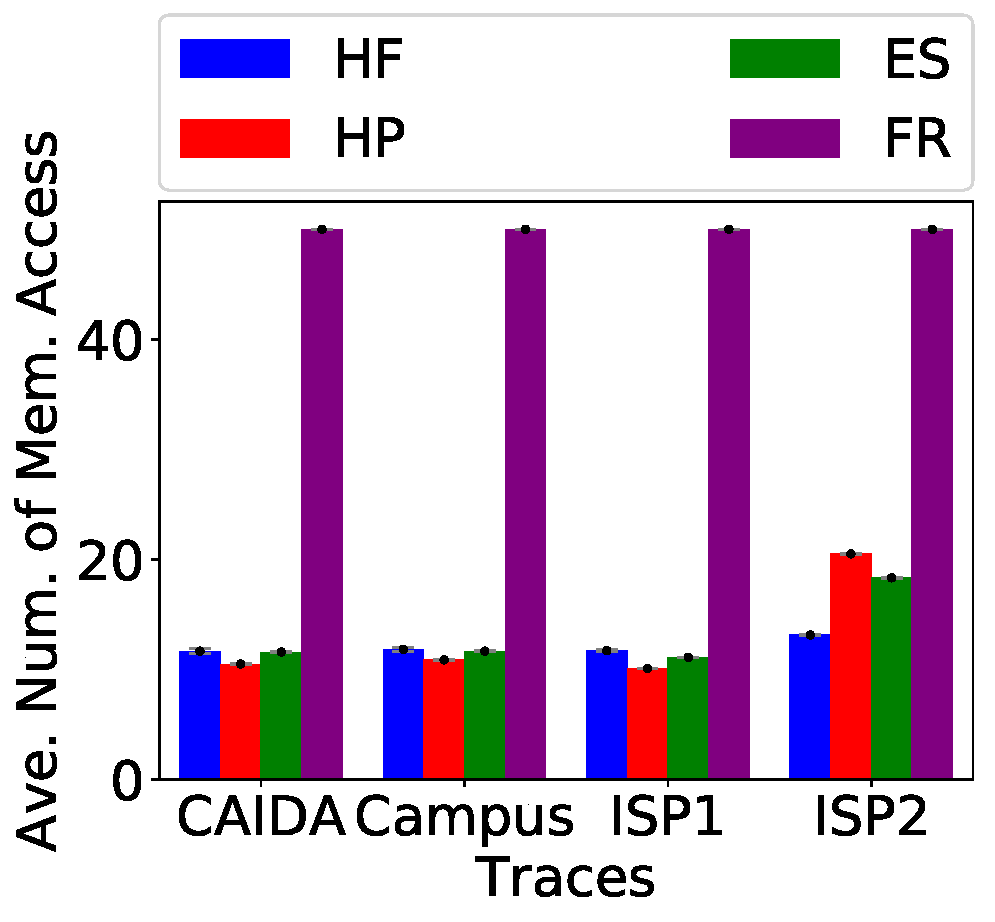
\includegraphics[width=0.9\linewidth]{figures/exp84490/ave_mem}
%    \caption{The average number of memory accesses for processing a packet.}
%    \label{fig:avemem}
%\end{figure}
\fi
